%=======================================================================
% Manuscript prepared for IEEE Transactions on Information Forensics
% and Security (TIFS) / adaptable to MDPI cybersecurity venues.
%=======================================================================
\documentclass[journal,twocolumn,10pt]{IEEEtran}

\usepackage{cite}
\usepackage{amsmath,amssymb,amsfonts}
\usepackage{algorithm}
\usepackage{algpseudocode}
\usepackage{graphicx}
\usepackage{booktabs}
\usepackage{multirow}
\usepackage{threeparttable}
\usepackage{xcolor}
\usepackage{tikz}
\usepackage{pgfplots}
\pgfplotsset{compat=1.16}
\usetikzlibrary{arrows.meta,positioning,shapes.geometric,fit,backgrounds}
\usepackage[hidelinks]{hyperref}
\usepackage{orcidlink}

% Path to the auto-generated analysis artifacts (tables, figures).
\newcommand{\analysis}{../experiment_validation/analysis}

\begin{document}

\title{A Cross-Model Evaluation of LLM Output Reconstruction from Token-Length Traces in Controlled SSE Streaming}

\author{Author~One,~\orcidlink{0000-0000-0000-0000}~\IEEEmembership{Member,~IEEE,}
        and~Author~Two,~\orcidlink{0000-0000-0000-0000}~\IEEEmembership{Senior~Member,~IEEE}
\thanks{Manuscript submitted \today. \emph{(Corresponding author: Author One.)}}
\thanks{The authors are with the Department/Institute, University/Organization, City, Country (e-mail: author1@example.com; author2@example.com).}
\thanks{Code, per-sample metrics, and a SHA-256 artifact manifest accompany this paper
(anonymous review mirror: \url{https://anonymous.4open.science/r/lleakm-repro-TBD}).}}

\markboth{IEEE Transactions on Information Forensics and Security,~Vol.~XX, No.~X, Month~2026}%
{Author One \MakeLowercase{\textit{et al.}}: Cross-Model Reconstruction from Controlled SSE Token-Length Traces}

\maketitle

\begin{abstract}
Large-language-model (LLM) assistants commonly stream responses token by token using Server-Sent Events (SSE). Frame sizes that remain observable under encryption can correlate with token lengths and thereby leak information about the generated text. This paper reports a \emph{controlled} cross-model evaluation of output reconstruction from \emph{idealized} one-token-per-frame length traces across seven open-weight language models (six instruction/chat-tuned models and one base model; 300 aligned prompts each; 2100 samples). A shared Weiss-style T5 pipeline recovers text hypotheses from length sequences. We score reconstructions with a single fixed \emph{term-frequency cosine similarity} $\phi$ (a lexical overlap measure, not a paraphrase-aware semantic embedding) and report the lexical recovery rate $\mathrm{LR}@0.5$ as the fraction of samples with $\phi>0.5$. Beyond point estimates we report bootstrap 95\% confidence intervals and paired Wilcoxon tests with Holm--Bonferroni correction. Mean $\phi$ varies significantly across models---from $0.324$ (Qwen2.5-1.5B-Instruct, 95\% CI $[0.310,0.338]$) to $0.024$ (Phi-3.5-mini-instruct)---and 19 of 21 pairwise differences remain significant after correction. We interpret the ranking as transferability of a fixed reconstructor onto each model's traces, report response-length covariates, and show via a linear model that model identity retains explanatory power after controlling for length and truncation. Trace-information baselines (shuffled, constant, and cross-prompt lengths) quantify how much signal the real length sequence contributes beyond the reconstructor's language prior. We further evaluate five transport-preserving defenses (four mechanism classes: bucketing, fixed framing, batching, randomized padding) \emph{against the fixed, non-adaptive reconstructor}, reporting residual $\phi$, Wilson intervals for $\mathrm{LR}@0.5$, and byte overhead---not only frame counts. No defended sample exceeded $\phi=0.5$ in the evaluated subset ($n=30$ prompts $\times$ 2 models; Wilson upper bounds remain nontrivial). End-to-end TLS extraction and adaptive attackers trained on defended traces are left to future work.
\end{abstract}

\begin{IEEEkeywords}
Large language models, side-channel analysis, server-sent events, traffic analysis, privacy leakage, token streaming, text reconstruction, statistical significance, defenses.
\end{IEEEkeywords}

\section{Introduction}
\IEEEPARstart{I}{nteractive} LLM assistants return answers incrementally to reduce perceived latency. A frequent pattern is token streaming over SSE, where each chunk is encapsulated in a frame transmitted over an encrypted transport. Encryption protects payload \emph{content}, but observable sizes can correlate with token lengths~\cite{weiss2024prompt}.

Weiss \emph{et al.} demonstrated token-length reconstruction on live ChatGPT and Copilot traffic (27\% response recovery; 53\% topic inference under their criteria)~\cite{weiss2024prompt}. Concurrent work studies merged API outputs~\cite{li2026length} and related streaming metadata attacks~\cite{whisperleak2025}. We ask a complementary question: under a controlled, idealized one-token-per-frame observation model, how does reconstruction quality vary across open-weight models when prompts, decoding, reconstructor, and metrics are held fixed?

\textbf{Scope.} We study an \emph{ideal token-length oracle} from an instrumented harness, not TLS ciphertext extraction. This provides an \emph{optimistic observation model} for a length-only adversary; bridging to live encrypted traffic remains future work (Section~\ref{sec:threat}).

\textbf{Contributions.}
\begin{enumerate}
\item A controlled cross-model reconstruction benchmark on aligned traces from seven open-weight models, with a fixed lexical scoring backend (Sections~\ref{sec:method}--\ref{sec:results}).
\item Uncertainty-aware claims: bootstrap CIs, paired Wilcoxon tests with Holm correction, effect sizes, length covariates, and a regression controlling for those covariates.
\item Trace-information baselines (shuffled / constant / cross-prompt) separating length-channel signal from reconstructor priors (Section~\ref{sec:baselines}).
\item Defense evaluation of five configurations against a \emph{fixed non-adaptive} reconstructor, with byte overhead and Wilson intervals for $\mathrm{LR}@0.5$ (Section~\ref{sec:defense}).
\item A reproducibility package with hashed artifacts (Section~\ref{sec:repro}).
\end{enumerate}

\section{Related Work}
Side-channel attacks exploit timing, size, and related observables~\cite{kocher1996timing,song2001timing,chen2010sidechannel}. Website fingerprinting and traffic-morphing defenses motivate size-domain mitigations~\cite{cai2012touching,sirinam2018deep,dyer2012peekaboo,wright2009morphing}. Weiss \emph{et al.} introduced LLM token-length reconstruction with known-plaintext fine-tuning on live traffic~\cite{weiss2024prompt}. Li \emph{et al.} study merged token packets~\cite{li2026length}. Our focus is a controlled multi-model benchmark under idealized traces, with statistical testing, trace baselines, and a non-adaptive defense sweep---not a new remote exploit.

\section{Threat Model and Experimental Scope}\label{sec:threat}
We study an adversary who obtains per-token UTF-8 lengths $L^{\mathrm{tok}}_1,\dots,L^{\mathrm{tok}}_n$ and reconstructs the response (Fig.~\ref{fig:threat}). In our harness, $L^{\mathrm{tok}}_t=L^{\mathrm{frame}}_t-8$ for SSE frames \texttt{data: <token>\textbackslash n\textbackslash n}. Reconstruction uses only the length sequence.

This matches the token-length \emph{channel abstraction} of Weiss \emph{et al.}~\cite{weiss2024prompt}, but lengths come from an instrumented one-token-per-frame server. A network adversary would still need to recover comparable lengths from TLS/HTTP/2/QUIC records that may coalesce, fragment, or pad frames. We therefore claim reconstructability under an idealized oracle, which is optimistic relative to ciphertext-only observation.

\begin{figure}[t]
\centering
\resizebox{\columnwidth}{!}{%
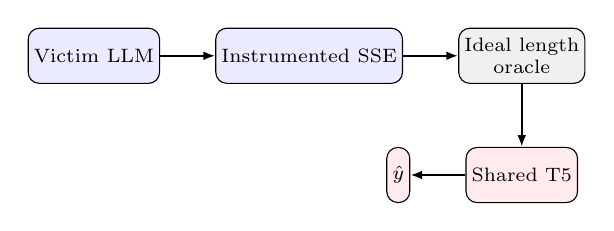
\begin{tikzpicture}[
  node distance=5mm and 7mm, font=\scriptsize,
  box/.style={draw,rounded corners,align=center,minimum height=7mm,inner sep=2pt},
  server/.style={box,fill=blue!8},
  attacker/.style={box,fill=red!8},
  wire/.style={-{Latex[length=1.5mm]},thick}]
  \node[server] (victim) {Victim LLM};
  \node[server,right=of victim] (sse) {Instrumented SSE};
  \node[box,right=of sse,fill=gray!12] (oracle) {Ideal length\\oracle};
  \node[attacker,below=8mm of oracle] (rec) {Shared T5};
  \node[attacker,left=of rec] (out) {$\hat{y}$};
  \draw[wire] (victim) -- (sse);
  \draw[wire] (sse) -- (oracle);
  \draw[wire] (oracle) -- (rec);
  \draw[wire] (rec) -- (out);
\end{tikzpicture}}
\caption{Ideal length oracle from an instrumented harness (not TLS capture).}
\label{fig:threat}
\end{figure}

\section{Materials and Methods}\label{sec:method}
\subsection{Harness and Trace Collection}
The harness emits one token per SSE frame and logs token UTF-8 length, frame length, and timestamps. Token text is retained only for auditing and offline metric recomputation.

\subsection{Reconstruction Pipeline}
We use \texttt{royweiss1/T5\_FirstSentences} and \texttt{royweiss1/T5\_MiddleSentences} without per-model fine-tuning (Algorithm~\ref{alg:recon}). Candidates are ranked by the unnormalized sum of transition log-probabilities (shorter candidates can be favoured). Cross-model differences therefore measure \emph{transfer} of this fixed reconstructor~\cite{weiss2024prompt}.

\textbf{Segmentation rules} (implemented in \texttt{weiss\_reconstruction.py}): (1)~split after every length-$1$ token (treated as punctuation under the Weiss heuristic); (2)~move a trailing $(3,1,1)$ list marker onto the next segment; (3)~merge any segment with fewer than $10$ tokens into the following segment; (4)~the final remainder forms its own segment. A length-$1$ token is not guaranteed to be sentence-final across tokenizers; the rule is part of the fixed attack configuration.

\begin{algorithm}[t]
\caption{Weiss-style reconstruction from length traces}
\label{alg:recon}
\begin{algorithmic}[1]
\Require lengths $L=(L^{\mathrm{tok}}_1,\dots,L^{\mathrm{tok}}_n)$
\State $S \gets \textsc{SegmentSentences}(L)$ \Comment{rules above}
\State decode first segment with T5-First; middle segments with T5-Middle
\State \Return concatenated top-ranked hypothesis $\hat{y}$
\end{algorithmic}
\end{algorithm}

\subsection{Models and Protocol}
Seven open-weight models: six instruction/chat-tuned and one base model (Phi-1.5). Primary comparative claims use the six instruction/chat models; Phi-1.5 is retained as a stress test (Table~\ref{tab:metadata}). Shared settings: $N=300$ aligned prompts, temperature~$0$, top-$p=1$, max-new-tokens~$96$, three samples per segment, and at most three sentences. Truncation rates of 95--100\% mean nearly all answers are cut mid-stream; results characterize early-response reconstructability under a tight budget.

\begin{table}[t]
\centering
\caption{Model metadata. Kind: instruct/chat vs.\ base.}
\label{tab:metadata}
\begin{threeparttable}
\footnotesize
\begin{tabular}{l c c l}
\toprule
Model & Params & Kind & Tokenizer family \\
\midrule
Qwen2.5-1.5B-Instruct & $\sim$1.5B & instruct & Qwen2 \\
Qwen2.5-3B-Instruct & $\sim$3B & instruct & Qwen2 \\
Llama-3.2-3B-Instruct & $\sim$3B & instruct & Llama \\
Gemma-2-2B-it & $\sim$2B & instruct & Gemma \\
Phi-1.5 & $\sim$1.3B & base & CodeGen \\
TinyLlama-1.1B-Chat & $\sim$1.1B & chat & Llama \\
Phi-3.5-mini-instruct & $\sim$3.8B & instruct & Llama \\
\bottomrule
\end{tabular}
\end{threeparttable}
\end{table}

\subsection{Metrics: Lexical Cosine $\phi$ and $\mathrm{LR}@0.5$}
We recompute for every sample a \emph{term-frequency cosine similarity} $\phi$ between bag-of-words vectors of the reference and the hypothesis ($\uparrow$). This measures lexical overlap; it is \emph{not} Sentence-BERT or BERTScore and can assign high scores to lexically similar but semantically wrong text (and vice versa). We avoid calling $\phi$ ``semantic similarity.''

The lexical recovery rate $\mathrm{LR}@0.5$ ($\uparrow$) is the fraction of samples with $\phi>0.5$ (Wilson CI). The threshold is conventional, not human-calibrated. We also report $ed_{\mathrm{norm}}$ ($\downarrow$) and ROUGE-1/L precision ($\uparrow$)~\cite{levenshtein1966binary,lin2004rouge}.

\subsection{Statistics}\label{sec:stats}
Bootstrap 95\% CIs ($B=10{,}000$) for means; Wilson intervals for $\mathrm{LR}@0.5$; paired Wilcoxon tests on per-prompt $\phi$ with Holm--Bonferroni over $\binom{7}{2}=21$ pairs and rank-biserial $r$~\cite{efron1994bootstrap,wilcoxon1945individual,holm1979simple}. Seed: \texttt{20260706}.

\section{Results}\label{sec:results}
\subsection{Control Covariates}
Table~\ref{tab:controls} shows mean/median token counts, characters, mean token UTF-8 bytes, and truncation. Equal token budgets do not imply equal text across tokenizers.

\begin{table}[t]
\centering
\caption{Control covariates ($N=300$). Trunc.\,\%: responses with $\geq$96 tokens.}
\label{tab:controls}
\footnotesize
\begin{tabular}{lccccccc}
\toprule
Model & Par. & Kind & Mean tok & Med. & Chars & Mean B/tok & Tr.\% \\
\midrule
% Auto-generated control covariates
Qwen2.5-1.5B-Instruct & $\sim$1.5B & instruct & 92.2 & 96 & 464 & 5.03 & 95.0 \\
Qwen2.5-3B-Instruct & $\sim$3B & instruct & 96.0 & 96 & 482 & 5.03 & 100.0 \\
Llama-3.2-3B-Instruct & $\sim$3B & instruct & 94.7 & 96 & 463 & 4.88 & 96.3 \\
Gemma-2-2B-it & $\sim$2B & instruct & 96.0 & 96 & 435 & 4.53 & 100.0 \\
Phi-1.5 & $\sim$1.3B & base & 96.0 & 96 & 497 & 5.17 & 99.7 \\
TinyLlama-1.1B-Chat & $\sim$1.1B & chat & 96.0 & 96 & 331 & 3.45 & 100.0 \\
Phi-3.5-mini-instruct & $\sim$3.8B & instruct & 96.0 & 96 & 342 & 3.57 & 100.0 \\

\bottomrule
\end{tabular}
\end{table}

\subsection{Cross-Model Comparison}
Table~\ref{tab:main} and Fig.~\ref{fig:phici} report $\phi$ with CIs (all seven models). Among instruction/chat models only (Table~\ref{tab:main_instruct}), the same ordering of extremes holds. Phi-1.5 ranks high under lexical cosine despite being a base model---consistent with reconstructor transfer, not chat alignment.

\begin{table*}[t]
\centering
\caption{All models ($N=300$). $\phi$: TF cosine ($\uparrow$); $ed_{\mathrm{norm}}$ ($\downarrow$); $\mathrm{LR}@0.5$ ($\uparrow$, \%).}
\label{tab:main}
\begin{threeparttable}
\footnotesize
\begin{tabular}{l c c c c c c}
\toprule
Model & $\phi\uparrow$ & 95\% CI & $ed\downarrow$ & R1$\uparrow$ & RL$\uparrow$ & $\mathrm{LR}@0.5$ \\
\midrule
% Auto-generated by analyze_stats.py -- main per-model table body
Qwen2.5-1.5B-Instruct & 0.3242 & $[0.3097, 0.3380]$ & 0.7199 & 0.3220 & 0.2651 & 8.67 $[5.98, 12.40]$ \\
Qwen2.5-3B-Instruct & 0.3096 & $[0.2977, 0.3214]$ & 0.7300 & 0.2945 & 0.2345 & 3.00 $[1.59, 5.60]$ \\
Phi-1.5 & 0.2747 & $[0.2622, 0.2877]$ & 0.7426 & 0.2503 & 0.1891 & 4.33 $[2.55, 7.27]$ \\
Llama-3.2-3B-Instruct & 0.2538 & $[0.2419, 0.2658]$ & 0.7499 & 0.2387 & 0.1824 & 3.00 $[1.59, 5.60]$ \\
Gemma-2-2B-it & 0.1798 & $[0.1708, 0.1889]$ & 0.7764 & 0.1719 & 0.1269 & 0.00 $[0.00, 1.26]$ \\
TinyLlama-1.1B-Chat & 0.0428 & $[0.0377, 0.0479]$ & 0.8026 & 0.0312 & 0.0310 & 0.00 $[0.00, 1.26]$ \\
Phi-3.5-mini-instruct & 0.0239 & $[0.0201, 0.0280]$ & 0.8087 & 0.0158 & 0.0157 & 0.00 $[0.00, 1.26]$ \\

\bottomrule
\end{tabular}
\end{threeparttable}
\end{table*}

\begin{table}[t]
\centering
\caption{Instruction/chat models only (Phi-1.5 excluded).}
\label{tab:main_instruct}
\footnotesize
\begin{tabular}{l c c c c c}
\toprule
Model & $\phi\uparrow$ & 95\% CI & $ed\downarrow$ & R1$\uparrow$ & $\mathrm{LR}@0.5$ \\
\midrule
% Instruct/chat models only (Phi-1.5 excluded)
Qwen2.5-1.5B-Instruct & 0.3242 & $[0.3097, 0.3380]$ & 0.7199 & 0.3220 & 8.67 $[5.98, 12.40]$ \\
Qwen2.5-3B-Instruct & 0.3096 & $[0.2977, 0.3214]$ & 0.7300 & 0.2945 & 3.00 $[1.59, 5.60]$ \\
Llama-3.2-3B-Instruct & 0.2538 & $[0.2419, 0.2658]$ & 0.7499 & 0.2387 & 3.00 $[1.59, 5.60]$ \\
Gemma-2-2B-it & 0.1798 & $[0.1708, 0.1889]$ & 0.7764 & 0.1719 & 0.00 $[0.00, 1.26]$ \\
TinyLlama-1.1B-Chat & 0.0428 & $[0.0377, 0.0479]$ & 0.8026 & 0.0312 & 0.00 $[0.00, 1.26]$ \\
Phi-3.5-mini-instruct & 0.0239 & $[0.0201, 0.0280]$ & 0.8087 & 0.0158 & 0.00 $[0.00, 1.26]$ \\

\bottomrule
\end{tabular}
\end{table}

\begin{figure}[t]
\centering
\resizebox{\columnwidth}{!}{% Auto-generated by make_figures.py -- phi with 95% bootstrap CI
\pgfplotsset{width=\linewidth,height=6cm,compat=1.16}
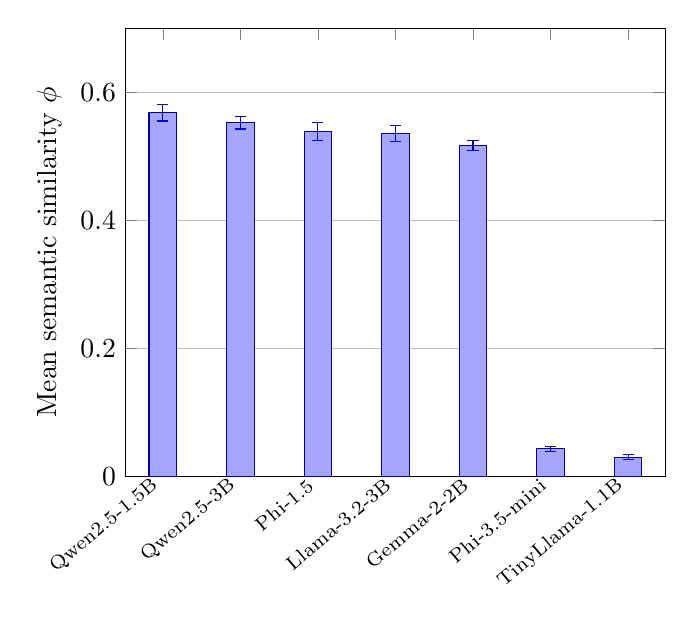
\begin{tikzpicture}
\begin{axis}[
  ybar, bar width=10pt, ymin=0, ymax=0.70,
  ylabel={Mean semantic similarity $\phi$},
  xtick={0,1,2,3,4,5,6},
  xticklabels={{Qwen2.5-1.5B},{Qwen2.5-3B},{Phi-1.5},{Llama-3.2-3B},{Gemma-2-2B},{Phi-3.5-mini},{TinyLlama-1.1B}},
  x tick label style={rotate=40,anchor=east,font=\scriptsize},
  enlarge x limits=0.08, ymajorgrids, tick align=inside,
]
\addplot+[ybar, fill=blue!35, draw=blue!60!black,
  error bars/.cd, y dir=both, y explicit] coordinates {
  (0,0.5680) +- (0.0130,0.0129) (1,0.5521) +- (0.0094,0.0094) (2,0.5383) +- (0.0133,0.0138) (3,0.5360) +- (0.0122,0.0126) (4,0.5170) +- (0.0084,0.0081) (5,0.0434) +- (0.0043,0.0041) (6,0.0302) +- (0.0038,0.0035)
};
\end{axis}
\end{tikzpicture}
}
\caption{Mean TF-cosine $\phi$ with 95\% bootstrap CIs ($N=300$).}
\label{fig:phici}
\end{figure}

\subsection{Significance and Covariate Control}
Table~\ref{tab:pairwise}: 19/21 pairs significant after Holm correction. A linear model $\phi=\beta_0+\beta_{\mathrm{model}}+\beta_1(\mathrm{chars}/100)+\beta_2\overline{|t|}+\beta_3\mathrm{trunc}$ on the six instruction/chat models yields $R^2=0.646$, versus $0.642$ for model indicators alone and $0.511$ for covariates alone (Table~\ref{tab:regression}). Model identity retains nearly all explanatory power after length controls; covariates alone are insufficient to explain the ranking.

\begin{table*}[t]
\centering
\caption{Paired Wilcoxon tests on $\phi$ ($n=300$). $^{*}$: $p_{\mathrm{Holm}}<0.05$.}
\label{tab:pairwise}
\footnotesize
\begin{tabular}{l c c c c c}
\toprule
Comparison & $\Delta\phi$ & 95\% CI & $r$ & $p_{\mathrm{raw}}$ & $p_{\mathrm{Holm}}$ \\
\midrule
% Auto-generated by analyze_stats.py -- pairwise Wilcoxon table body
Qwen2.5-1.5B-Instruct vs.\ Gemma-2-2B-it & +0.1443 & $[+0.1276, +0.1608]$ & +0.837 & $<$0.0001 & $<$0.0001$^{*}$ \\
Qwen2.5-1.5B-Instruct vs.\ TinyLlama-1.1B-Chat & +0.2814 & $[+0.2660, +0.2967]$ & +0.999 & $<$0.0001 & $<$0.0001$^{*}$ \\
Qwen2.5-1.5B-Instruct vs.\ Phi-3.5-mini-instruct & +0.3002 & $[+0.2851, +0.3152]$ & +1.000 & $<$0.0001 & $<$0.0001$^{*}$ \\
Qwen2.5-3B-Instruct vs.\ Gemma-2-2B-it & +0.1297 & $[+0.1145, +0.1450]$ & +0.826 & $<$0.0001 & $<$0.0001$^{*}$ \\
Qwen2.5-3B-Instruct vs.\ TinyLlama-1.1B-Chat & +0.2668 & $[+0.2542, +0.2795]$ & +1.000 & $<$0.0001 & $<$0.0001$^{*}$ \\
Qwen2.5-3B-Instruct vs.\ Phi-3.5-mini-instruct & +0.2856 & $[+0.2727, +0.2985]$ & +1.000 & $<$0.0001 & $<$0.0001$^{*}$ \\
Llama-3.2-3B-Instruct vs.\ Gemma-2-2B-it & +0.0739 & $[+0.0595, +0.0889]$ & +0.566 & $<$0.0001 & $<$0.0001$^{*}$ \\
Llama-3.2-3B-Instruct vs.\ TinyLlama-1.1B-Chat & +0.2110 & $[+0.1978, +0.2244]$ & +0.994 & $<$0.0001 & $<$0.0001$^{*}$ \\
Llama-3.2-3B-Instruct vs.\ Phi-3.5-mini-instruct & +0.2298 & $[+0.2168, +0.2430]$ & +0.998 & $<$0.0001 & $<$0.0001$^{*}$ \\
Gemma-2-2B-it vs.\ Phi-1.5 & -0.0948 & $[-0.1105, -0.0792]$ & -0.681 & $<$0.0001 & $<$0.0001$^{*}$ \\
Gemma-2-2B-it vs.\ TinyLlama-1.1B-Chat & +0.1370 & $[+0.1268, +0.1472]$ & +0.977 & $<$0.0001 & $<$0.0001$^{*}$ \\
Gemma-2-2B-it vs.\ Phi-3.5-mini-instruct & +0.1559 & $[+0.1457, +0.1663]$ & +0.990 & $<$0.0001 & $<$0.0001$^{*}$ \\
Phi-1.5 vs.\ TinyLlama-1.1B-Chat & +0.2319 & $[+0.2179, +0.2459]$ & +0.998 & $<$0.0001 & $<$0.0001$^{*}$ \\
Phi-1.5 vs.\ Phi-3.5-mini-instruct & +0.2507 & $[+0.2367, +0.2649]$ & +0.999 & $<$0.0001 & $<$0.0001$^{*}$ \\
Qwen2.5-1.5B-Instruct vs.\ Llama-3.2-3B-Instruct & +0.0704 & $[+0.0530, +0.0875]$ & +0.498 & $<$0.0001 & $<$0.0001$^{*}$ \\
Qwen2.5-3B-Instruct vs.\ Llama-3.2-3B-Instruct & +0.0558 & $[+0.0394, +0.0719]$ & +0.426 & $<$0.0001 & $<$0.0001$^{*}$ \\
TinyLlama-1.1B-Chat vs.\ Phi-3.5-mini-instruct & +0.0189 & $[+0.0132, +0.0245]$ & +0.454 & $<$0.0001 & $<$0.0001$^{*}$ \\
Qwen2.5-1.5B-Instruct vs.\ Phi-1.5 & +0.0495 & $[+0.0305, +0.0686]$ & +0.330 & $<$0.0001 & $<$0.0001$^{*}$ \\
Qwen2.5-3B-Instruct vs.\ Phi-1.5 & +0.0349 & $[+0.0165, +0.0528]$ & +0.268 & $<$0.0001 & 0.0002$^{*}$ \\
Llama-3.2-3B-Instruct vs.\ Phi-1.5 & -0.0209 & $[-0.0375, -0.0043]$ & -0.148 & 0.0266 & 0.0533 \\
Qwen2.5-1.5B-Instruct vs.\ Qwen2.5-3B-Instruct & +0.0146 & $[-0.0026, +0.0314]$ & +0.089 & 0.1838 & 0.1838 \\

\bottomrule
\end{tabular}
\end{table*}

\begin{table}[t]
\centering
\caption{OLS fit for $\phi$ (instruct/chat models, $n=1800$).}
\label{tab:regression}
\footnotesize
\begin{tabular}{l c}
\toprule
Quantity & Value \\
\midrule
% Auto-generated covariate regression summary
Full model $R^2$ & 0.646 \\
Model indicators only $R^2$ & 0.642 \\
Covariates only (chars, token bytes, trunc.) $R^2$ & 0.511 \\
$\beta_{\mathrm{chars}/100}$ & -0.0179 \\
$\beta_{\mathrm{mean\,token\,bytes}}$ & +0.0290 \\
$\beta_{\mathrm{truncated}}$ & -0.0295 \\

\bottomrule
\end{tabular}
\end{table}

\section{Trace-Information Baselines}\label{sec:baselines}
To isolate the contribution of the length channel beyond the T5 language prior, we reconstruct from (i)~the real length sequence, (ii)~a within-response shuffle, (iii)~a constant sequence at the mean token length, and (iv)~a cross-prompt length sequence of equal cardinality, on the same topic-balanced subset used for defenses ($n=30$ prompts per model). Table~\ref{tab:baselines} shows that real traces outperform all degraded traces: shuffling lowers mean $\phi$ by about $0.09$--$0.10$, and a constant-length sequence lowers it by about $0.17$--$0.20$. Cross-prompt lengths remain closer to real ($\Delta\approx -0.05$ to $-0.06$), indicating that response length \emph{structure}---not only marginal length statistics---carries usable information under the fixed reconstructor.

\begin{table}[t]
\centering
\caption{Trace-information baselines (TF-cosine $\phi$). Negative $\Delta$ vs.\ real means the degraded trace yields lower lexical overlap.}
\label{tab:baselines}
\footnotesize
\begin{tabular}{l l c c c c}
\toprule
Model & Condition & $n$ & $\phi$ & 95\% CI & $\Delta$ vs.\ real \\
\midrule
Qwen2.5-1.5B-Instruct & real & 30 & 0.3024 & $[0.2607, 0.3457]$ & --- \\
 & shuffled & 30 & 0.2091 & $[0.1734, 0.2463]$ & $-0.0933$ \\
 & constant & 30 & 0.1068 & $[0.0844, 0.1303]$ & $-0.1957$ \\
 & cross\_prompt & 30 & 0.2561 & $[0.2296, 0.2837]$ & $-0.0463$ \\
\midrule
Llama-3.2-3B-Instruct & real & 30 & 0.2913 & $[0.2568, 0.3282]$ & --- \\
 & shuffled & 30 & 0.1872 & $[0.1623, 0.2119]$ & $-0.1041$ \\
 & constant & 30 & 0.1242 & $[0.0981, 0.1529]$ & $-0.1671$ \\
 & cross\_prompt & 30 & 0.2312 & $[0.2010, 0.2618]$ & $-0.0601$ \\
\bottomrule
\end{tabular}
\end{table}

\section{Defense Evaluation}\label{sec:defense}
\subsection{Defenses (Non-Adaptive Attacker)}
We evaluate \emph{five} defense configurations (four classes) that transform observable lengths before reconstruction with the \emph{same} undefended-trained T5 pipeline---i.e., a fixed, non-adaptive attacker who does not retrain on defended traces~\cite{weiss2024prompt,wright2009morphing}:
\begin{itemize}
\item \texttt{bucket\_8}: ceil each length to a multiple of 8;
\item \texttt{pad\_32}: online fixed frame size $C=32$ (no response-wide look-ahead; tokens longer than $C$ still emit size $C$);
\item \texttt{batch\_2} / \texttt{batch\_4}: one frame per $k$ tokens;
\item \texttt{rand\_pad\_8}: uniform padding in $\{0,\dots,8\}$ (seeded).
\end{itemize}
We do \emph{not} claim security against an adaptive adversary who fine-tunes on padded/batched traces.

\subsection{Results}
Table~\ref{tab:defense} reports residual $\phi$, $\mathrm{LR}@0.5$ with Wilson intervals, mean byte overhead
$\mathrm{OH}=100(\mathrm{bytes}_{\mathrm{def}}-\mathrm{bytes}_{\mathrm{base}})/\mathrm{bytes}_{\mathrm{base}}$,
and leakage reduction vs.\ each model's own baseline ($n=30$ topic-balanced prompts; Qwen2.5-1.5B and Llama-3.2-3B). No defended sample exceeded $\phi=0.5$ in this subset; Wilson upper bounds are about $11\%$, so ``zero observed successes'' must not be read as a point estimate of zero risk. Bucketing is the strongest among the tested options against the frozen reconstructor ($\approx$83--90\% $\phi$ reduction). Online \texttt{pad\_32} is weaker ($\approx$35--37\% reduction) despite very large byte overhead ($\approx$5--6$\times$), because a constant frame size still admits a trivial reconstruction prior when $C$ is far above typical token UTF-8 lengths; smaller online constants (e.g., $C\in\{8,16\}$) are a natural follow-up. Batching reduces frame count at zero byte sum overhead in our accounting and yields $\approx$68\% reduction; randomized padding sits in between.

\begin{table*}[t]
\centering
\caption{Defenses vs.\ fixed reconstructor ($n=30$/model). $\mathrm{LR}@0.5$ with Wilson 95\% CI; byte overhead \%; leak.\ reduction \%. Online fixed framing uses $C=32$.}
\label{tab:defense}
\begin{threeparttable}
\footnotesize
\begin{tabular}{l l c c c c c c}
\toprule
Model & Def. & $n$ & $\phi$ & 95\% CI & $\mathrm{LR}@0.5$ & Byte OH{\%} & Red.{\%} \\
\midrule
Qwen2.5-1.5B-Instruct & baseline & 30 & 0.3010 & $[0.2537, 0.3508]$ & 13.3 $[5.3, 29.7]$ & 0.0 & 0.0 \\
 & bucket\_8 & 30 & 0.0293 & $[0.0198, 0.0397]$ & 0.0 $[0.0, 11.4]$ & 82.4 & 90.3 \\
 & pad\_32 & 30 & 0.1901 & $[0.1667, 0.2150]$ & 0.0 $[0.0, 11.4]$ & 538.0 & 36.8 \\
 & batch\_2 & 30 & 0.0928 & $[0.0791, 0.1072]$ & 0.0 $[0.0, 11.4]$ & 0.0 & 69.2 \\
 & batch\_4 & 30 & 0.0950 & $[0.0668, 0.1269]$ & 0.0 $[0.0, 11.4]$ & 0.0 & 68.4 \\
 & rand\_pad\_8 & 30 & 0.1033 & $[0.0871, 0.1203]$ & 0.0 $[0.0, 11.4]$ & 81.6 & 65.7 \\
\midrule
Llama-3.2-3B-Instruct & baseline & 30 & 0.2576 & $[0.2177, 0.2978]$ & 3.3 $[0.6, 16.7]$ & 0.0 & 0.0 \\
 & bucket\_8 & 30 & 0.0428 & $[0.0305, 0.0563]$ & 0.0 $[0.0, 11.4]$ & 88.6 & 83.4 \\
 & pad\_32 & 30 & 0.1674 & $[0.1382, 0.2003]$ & 0.0 $[0.0, 11.4]$ & 565.1 & 35.0 \\
 & batch\_2 & 30 & 0.0823 & $[0.0684, 0.0967]$ & 0.0 $[0.0, 11.4]$ & 0.0 & 68.0 \\
 & batch\_4 & 30 & 0.0832 & $[0.0615, 0.1055]$ & 0.0 $[0.0, 11.4]$ & 0.0 & 67.7 \\
 & rand\_pad\_8 & 30 & 0.1004 & $[0.0834, 0.1186]$ & 0.0 $[0.0, 11.4]$ & 85.0 & 61.0 \\
\bottomrule
\end{tabular}
\begin{tablenotes}\footnotesize
\item Effectiveness is against the frozen baseline reconstructor only.
\end{tablenotes}
\end{threeparttable}
\end{table*}

\begin{figure}[t]
\centering
\resizebox{\columnwidth}{!}{% Auto-generated by make_figures.py -- residual phi per defense
\pgfplotsset{width=\linewidth,height=6cm,compat=1.16}
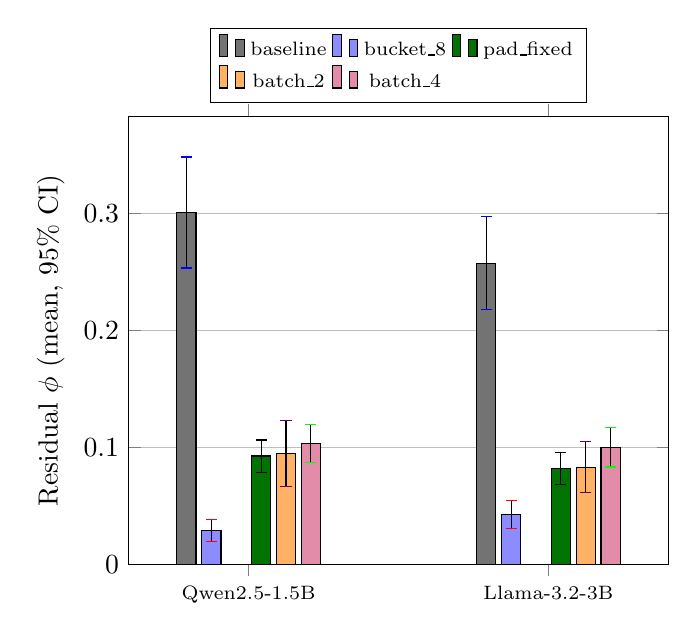
\begin{tikzpicture}
\begin{axis}[
  ybar, bar width=7pt, ymin=0,
  ylabel={Residual $\phi$ (mean, 95\% CI)},
  symbolic x coords={Qwen2.5-1.5B,Llama-3.2-3B},
  xtick=data, x tick label style={font=\scriptsize},
  legend style={font=\scriptsize,at={(0.5,1.03)},anchor=south,legend columns=3},
  ymajorgrids, enlarge x limits=0.4,
]
\addplot+[ybar,fill=black!55,draw=black,
  error bars/.cd, y dir=both, y explicit] coordinates {(Qwen2.5-1.5B,0.3010) +- (0.0498,0.0474) (Llama-3.2-3B,0.2576) +- (0.0402,0.0399)};
\addlegendentry{baseline}
\addplot+[ybar,fill=blue!45,draw=black,
  error bars/.cd, y dir=both, y explicit] coordinates {(Qwen2.5-1.5B,0.0293) +- (0.0104,0.0095) (Llama-3.2-3B,0.0428) +- (0.0135,0.0123)};
\addlegendentry{bucket\_8}
\addplot+[ybar,fill=red!45,draw=black,
  error bars/.cd, y dir=both, y explicit] coordinates {};
\addlegendentry{pad\_fixed}
\addplot+[ybar,fill=green!45!black,draw=black,
  error bars/.cd, y dir=both, y explicit] coordinates {(Qwen2.5-1.5B,0.0928) +- (0.0144,0.0137) (Llama-3.2-3B,0.0823) +- (0.0144,0.0139)};
\addlegendentry{batch\_2}
\addplot+[ybar,fill=orange!60,draw=black,
  error bars/.cd, y dir=both, y explicit] coordinates {(Qwen2.5-1.5B,0.0950) +- (0.0318,0.0283) (Llama-3.2-3B,0.0832) +- (0.0224,0.0217)};
\addlegendentry{batch\_4}
\addplot+[ybar,fill=purple!45,draw=black,
  error bars/.cd, y dir=both, y explicit] coordinates {(Qwen2.5-1.5B,0.1033) +- (0.0170,0.0162) (Llama-3.2-3B,0.1004) +- (0.0182,0.0170)};
\addlegendentry{rand\_pad\_8}
\end{axis}
\end{tikzpicture}
}
\caption{Residual $\phi$ (mean $\pm$ 95\% CI) under defenses (fixed reconstructor).}
\label{fig:defense}
\end{figure}

\section{Qualitative Examples}
Table~\ref{tab:qual} illustrates high and low TF-cosine cases. High $\phi$ can preserve boilerplate structure while altering key entities (career vs.\ barrister), underscoring that $\mathrm{LR}@0.5$ is a lexical---not semantic---proxy.

\begin{table}[t]
\centering
\caption{Illustrative reconstructions (truncated). Full strings in \texttt{qualitative\_examples.json}.}
\label{tab:qual}
\footnotesize
\begin{tabular}{l c p{0.28\columnwidth} p{0.28\columnwidth}}
\toprule
Model & $\phi$ & Reference (excerpt) & Hypothesis (excerpt) \\
\midrule
Qwen 1.5B & 0.69 & disclose a disability at work\ldots keep a journal & become a barrister in Ohio\ldots keep a journal \\
Qwen 1.5B & 0.08 & managing credit card debt\ldots budget plan & electric guitars\ldots advertising \\
\bottomrule
\end{tabular}
\end{table}

\section{Reproducibility}\label{sec:repro}
Scripts: \texttt{analyze\_stats.py}, \texttt{analyze\_extras.py}, \texttt{defense\_eval.py}, \texttt{trace\_baselines.py}, \texttt{make\_figures.py}, \texttt{make\_repro\_manifest.py}. Environment snapshot: \texttt{env\_snapshot.json}. Artifact hashes: \texttt{repro\_manifest.json}. Tables/figures are \texttt{\textbackslash input} from \texttt{experiment\_validation/analysis/}.

\section{Discussion}
Mean reconstructability under idealized traces varies significantly across the evaluated models. The ranking is reconstructor transfer, not intrinsic leakage after per-model adaptation. Defenses substantially reduced observed $\phi$ against the fixed reconstructor and yielded no $\mathrm{LR}@0.5$ successes in the pilot subset; they are \emph{promising mitigations against that attacker model}, not proven robust to adaptive retraining. High truncation under 96 tokens limits ecological validity; sensitivity runs at 256--384 tokens are recommended.

\section{Conclusion}
We presented a controlled cross-model evaluation of LLM output reconstruction from idealized SSE length traces, with lexical (not embedding) scoring, paired statistics, covariate analysis, trace baselines, and a five-configuration defense study against a non-adaptive reconstructor. Future work: live TLS extraction, adaptive defended-trace attackers, Sentence-BERT/BERTScore with human ratings, longer generation budgets, and multi-seed randomized padding.

\section*{Acknowledgment}
We thank the maintainers of the open models and the \texttt{royweiss1} checkpoints.

\appendix
\section{Topic Sensitivity (Exploratory)}
Best/worst topics ($N=20$/topic) for three models are exploratory only; full means are in \texttt{topic\_matrix.json}. No interaction test is claimed.
\begin{table}[t]
\centering
\caption{Exploratory best/worst topics by mean $\phi$.}
\label{tab:topic}
\footnotesize
\begin{tabular}{l l c l c}
\toprule
Model & Best & $\phi$ & Worst & $\phi$ \\
\midrule
% Auto-generated by analyze_stats.py -- topic sensitivity (best/worst)
Llama-3.2-3B-Instruct & employment & 0.3373 & safety\_security & 0.2053 \\
Gemma-2-2B-it & beliefs\_values & 0.2090 & financial\_status & 0.1575 \\
Phi-3.5-mini-instruct & financial\_status & 0.0444 & personal\_identity & 0.0073 \\

\bottomrule
\end{tabular}
\end{table}

\section{Environment}
Python/platform/package versions: see \texttt{env\_snapshot.json} (numpy, torch, transformers). Decoding: deterministic; chat templates follow each model's Hugging Face defaults.

\bibliographystyle{IEEEtran}
\bibliography{references}

\end{document}
